\subsection{Exploring Variants and Possible Improvements}

\MS{Adapt this intro or even the structure depending on other
  variants.}

Our simulation framework facilitates the simulation of variants of
placement algorithms. In the following, we present several variants of
the placement algorithms introduced in Sec.~\ref{sec:vm-schedulers}
that have been discussed in the literature or come up during the
implementation of their models using \vmps. This section provides
strong evidence that the modification and evaluation of existing
algorithms is much facilitated by our simulation framework.



% \subsubsection{Variants of hierarchical scheduling}
% \label{sec:snoozeVariants}

% We now present three non-trivial variants that we have implemented and
% explored: periodic vs.\ reactive scheduling, a variant of the
% assignment algorithm of LCs to GMs, and a variant of the algorithms of
% how GMs and LCs join the system.  \MS{How and where do we provide the
%   scheduling parameters for the evals.?}

\subsubsection{Hierarchical scheduling: periodic vs.\  reactive}

Snooze~\cite{feller:ccgrid12} schedules VMs in a periodic fashion:
after a fixed time period a GM calls the scheduler in order to resolve
resource conflicts among the LCs it manages. The information whether a
resource conflict has to be handled is taken based on the summary
information that is periodically sent by the LCs to the GM.

Using \vmps, we have also implemented an alternative, reactive,
strategy to scheduling: as soon as resource conflicts occur, LCs avert
their GMs of them; the GMs then immediately initiate
scheduling. Implementing this reactive scheme can be done using our
framework in two manners. First, by implementing additional
asynchronous transmissions of the necessary state updates as a real
implementation would proceed. Second, in a much more lightweight
manner through direct accesses by the GMs to the states of their
respective LCs. In order to ensure that this lightweight
implementation mimics a real implementation closely, delays induced by
communication in the ``real'' implementation are accounted for
explicitly (congestion issues are not relevant in this case because
notification of a resource conflict implies little communication and
conflict resolution blocks the GM and its LCs anyway). We have
implemented this lightweight variant of reactive scheduling including
an explicit model of communication delays. Using the abstractions
provided by \vmps, in particular harnessing its extended notion of
hosts that represent the VMs managed by the LCs of a VM, reactive
scheduling has been implemented by adding or modifying just 4~lines of
code of the variant with periodic scheduling.

{\scriptsize \begin{tabular}{|P{27mm}@{\:}||@{\:}c@{\:}|@{\:}c@{\:}|@{\:}c@{\:}||@{\:}c@{\:}|@{\:}c@{\:}|@{\:}c@{\:}|}
    \thickhline
    \textbf{Algorithm}
      & \multicolumn{3}{c@{\:}||@{\:}}{\textbf{No.\ migrations}}
      & \multicolumn{3}{c@{\:}|}{\textbf{Violation time (s)}}
        \Tstrut \\
       \hfill\#LCs  & ~128~ & ~256~ & 512 & ~~128~~ & ~~256~~ & 512 \Bstrut \\
    \thickhline
      Reactive      & 107 & 201 & 421 & 1075 & 1955 & 4385 \\
      Periodic 30s  & 62 & 124 & 269 & 1770 & 3453 & \:8196
    \Rstrut  \\ \hline
    \thickhline
\end{tabular} }

\AL[MS]{Update the table: it may make
sense to put all values to make the read and the understanding easier
Periodic 32 GMs, Reactive 32 GMs and finally DVMS}

We have shown the usefulness of our framework by exploring some
properties of reactive scheduling compared to periodic scheduling. To
this end we have simulated reactive scheduling and a periodic
algorithm for configurations ranging from 128 to 512~LCs. In each case
the Entropy scheduler has been applied on groups of 32~LCs per GM. The
periodic strategy has computed and applied reconfiguration plans every
30 secs. These simulations have yielded the results shown in the table
above. They clearly show that, while a reactive strategy entails a
much higher number of migrations (because the periodic one aggregates
overload situations and misses some of them), reactive scheduling
results in a significantly lower total migration time. \AL[MS]{lower
  total migration time ? you mean violation time, please correct.}

\begin{figure*}
\subcapcentertrue
\subfigure[DVMS]{
  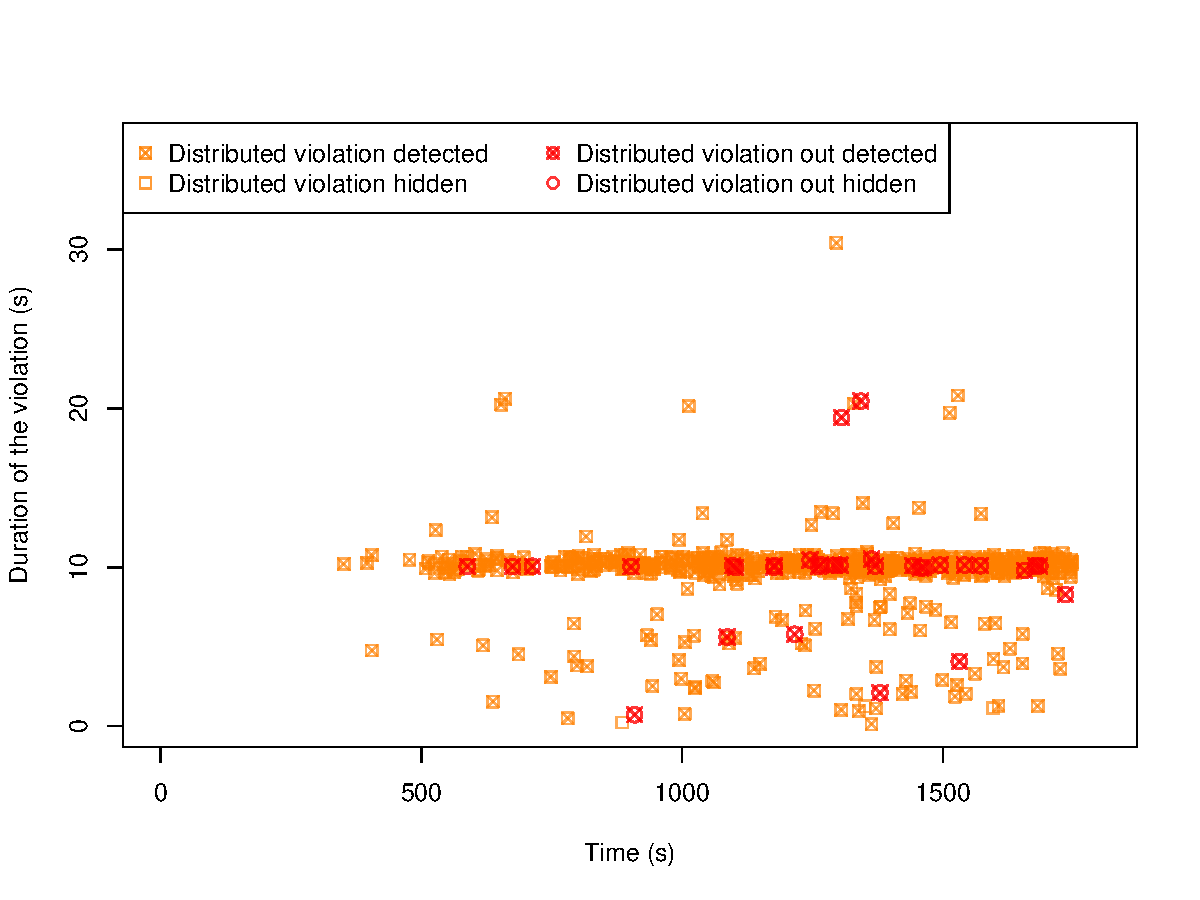
\includegraphics[width=.32\linewidth]{figures/experiments/clouds-1024-distributed.pdf}
  \label{fig:violation_clouds_dvms_1024}}
\subfigure[Snooze Periodic]{
  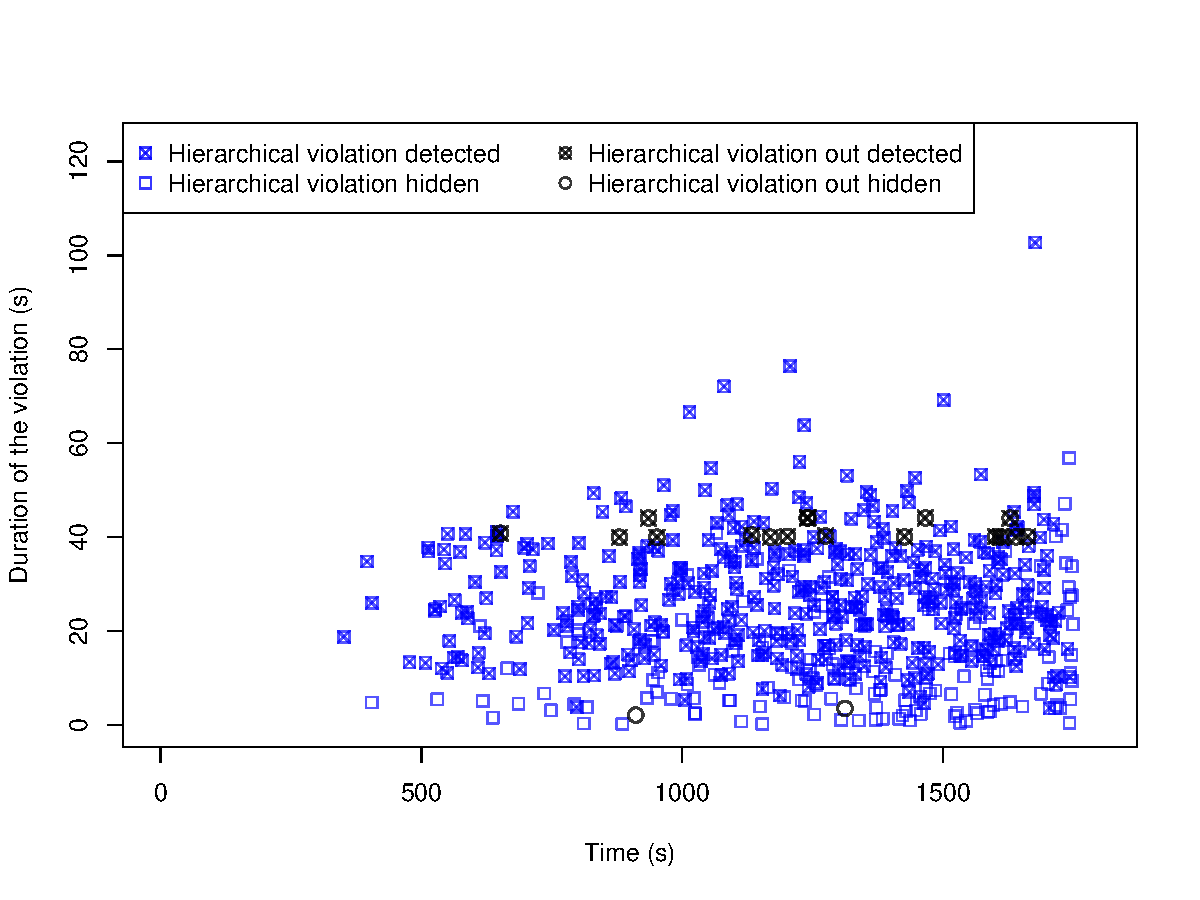
\includegraphics[width=.32\linewidth]{figures/experiments/clouds-1024-hierarchical-periodic-30-gm32.pdf}
  \label{fig:violation_clouds_snooze_1024_periodic}}
\subfigure[Snooze Reactive]{
  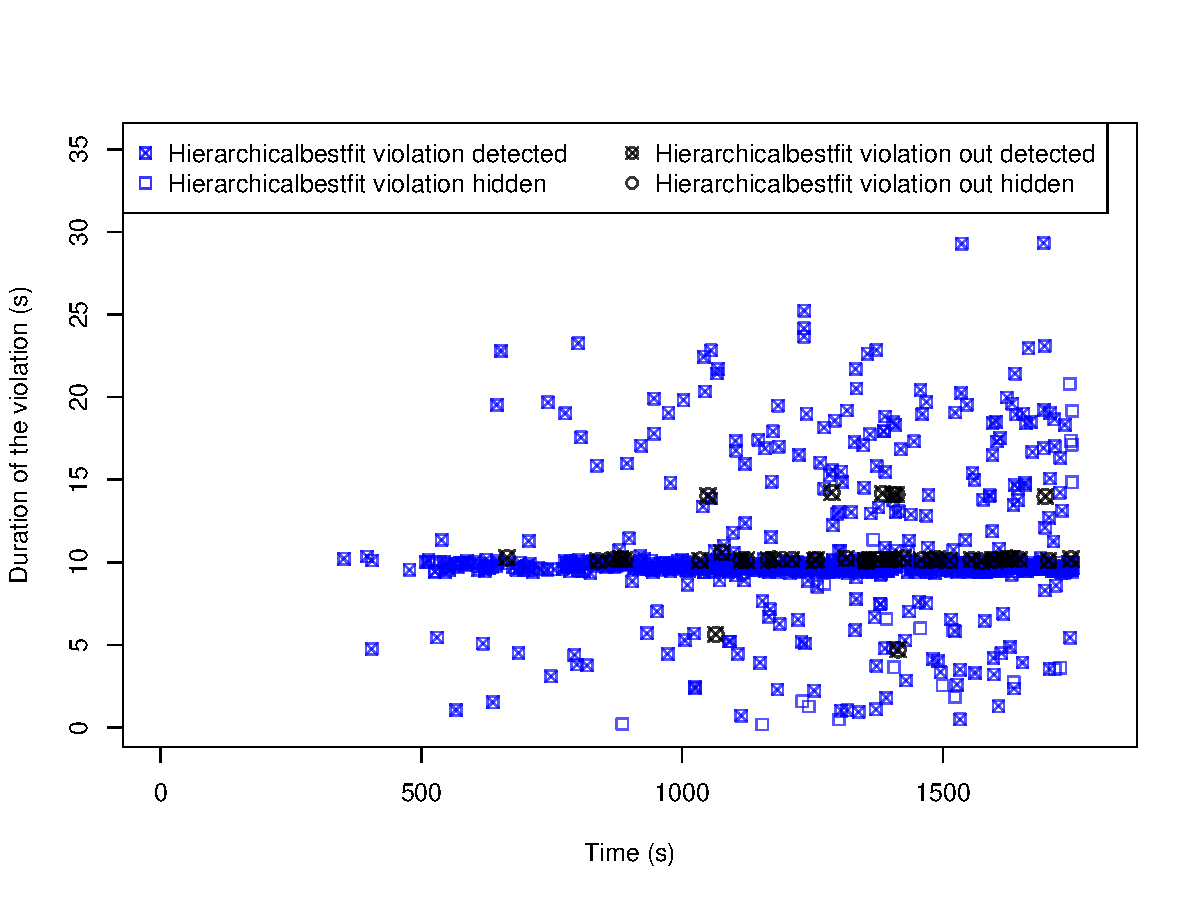
\includegraphics[width=.32\linewidth]{figures/experiments/clouds-1024-hierarchical-reactive-gm32.pdf}
  \label{fig:violation_clouds_snooze_1024_reactive}}
\caption{Details of violations duration occuring during simulation (10240 VMS).}
\label{fig:violation_clouds}
\end{figure*}
\AL[AL]{Figure \ref{fig:violation_clouds} should be discussed after
  the reactive discussion, the figure illustrates the pros of the reactivity.}
% \paragraph{Assignment of LCs to GMs}

% LCs are assigned to GMs by the GL as part of the LC join protocol. In
% Snooze's native implementation LCs are assigned in a round-robin
% fashion to the known GMs. If GMs join (and leave) the system at the
% same time as LCs, a round-robin (RR) strategy at join time, however,
% does not ensure an even distribution. This may happen, for instance at
% startup time of the system, when new GMs and LCs enter the system, or
% in case of failures, which trigger GM and LC joins. In order to
% evaluate the corresponding imbalance and its consequences we have
% implemented the LC assignment protocol in a modular fashion and
% applied it to different highly-dynamic settings in which GMs and LCs
% enter the system at the same time. Furthermore, we have implemented a
% best-fit (BF) strategy that assigns LCs to the GMs with minimal load
% or, if several GMs with minimal load exist, to the GMs with the
% smallest number of assigned LCs.


% % \subsubsection{LC assignment in Snooze-like placement alg.}
% % \label{sec:snoozeVariantsEval}

% % \begin{figure}[ht]
% % \begin{center}
% %     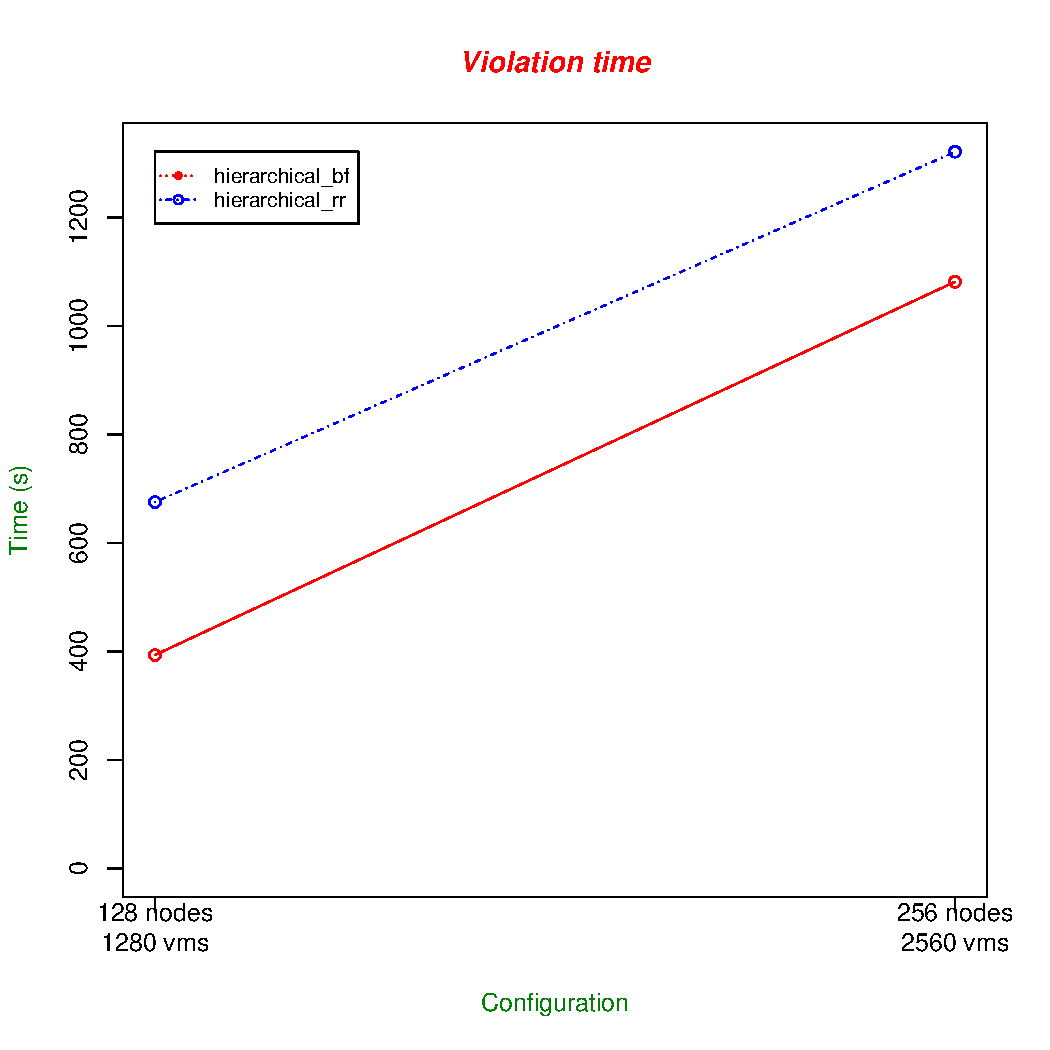
\includegraphics[width=.95\linewidth]{figures/violationTime-snooze-RR-BF.pdf}
% %     \caption{Cumulated violation time for BF (lower line) and RR
% %       (upper line) variants}
% % \end{center}
% % \label{fig:snoozeBFRRViolation}
% \end{figure}

% \begin{table*}[ht]
% \begin{center}
% %    \begin{tabular}{|c!{\vrule width 3pt}c|c|c!{\vrule width 2pt}c|c|c!{\vrule width 3pt}c|c!{\vrule width 2pt}c|c|}
%     \begin{tabular}{|P{30mm}|||c|c||c|c|||M{30mm}|M{30mm}|}
%         \thickhline
%         \multirow{3}*{\textbf{Strategy}}
%           & \multicolumn{4}{c|||}{\textbf{\#LCs/\#GMs}}
%           & \multicolumn{2}{c|}{\textbf{Total violation time (s)}}
%           \Tstrut \\
%           & \multicolumn{2}{c||}{128 LCs, 12 GMs}
%             & \multicolumn{2}{c|||}{256 LCs, 25 GMs}
%           & \multirow{2}*{128 LCs, 12 GMs} & \multirow{2}*{256 LCs, 25 GMs}
%           \Bstrut \\
%           & range & stdev & range & stdev & &  \Bstrut \\
%         \thickhline
%         Best-Fit & 0--30 & 10.53 & 0--18 & 6.62  & 395 & 1005 \Rstrut \\
%         Round-Robin & 0--49 & 15.7  & 0--35 & 12.22 & 630 & 1265
%         \Rstrut \\ \hline
%         \thickhline
%     \end{tabular}
% \end{center}
%     \caption{LCs to GM assignment and cumulated violation times for RR
%       and BF strategies}
%     \label{tbl:assignmentResults}
% \end{table*}


% We have evaluated the two LC assignment strategies using \vmps on
% configurations of~128 and~256 nodes. In order to clearly expose the
% corresponding differences this evaluation has been performed by
% ``stressing'' the two strategies by simultaneously
% starting all LCs (128/256) and all GMs (12/25) and then simulating the
% resulting configuration over a one hour period.  These experiments
% have yielded the following results, cf.\ Table~\ref{tbl:assignmentResults}:
% \begin{itemize}
%   \item BF yields more homogeneous assignments of LCs to GMs: the
%     ranges of the numbers of LCs assigned to a GM and their standard
%     deviations are significantly smaller.\footnote{Here, some GMs may
%       be assigned 0 LCs if some GMs join the system after all LCs have
%       been assigned.}
%   \item The cumulated time spent resolving violations is, for both
%     configurations, significantly smaller for BF than for RR.
% \end{itemize}
% From these results, we can clearly infer that BF is significantly
% better than RR for the two tested kinds of configuration. Furthermore,
% we conjecture that BF should perform at least as good as RR for all
% configurations (the proof is left to future work).
% % \MS[JP]{I need the exact figures for the violation times
% %   in Tbl.~\ref{tbl:assignmenResults}}

% \paragraph{Variants of the join algorithms}

% The join algorithms, see Sec.~\ref{sec:snoozeAlgs}, are crucial to
% Snooze for two main reasons: (i) they have to be efficient because
% they can easily form a bottleneck if large numbers of LCs (GMs) have
% to be registered at a GM (LC); (ii) they are multi-phase protocols
% whose correctness especially in the presence of faults is difficult to
% ensure.

% In order to investigate the corresponding trade-offs, we have used our
% framework to implement join algorithms that may be interrupted at any
% time, repeat the the on-going phase a number of times before
% reinitiating, if necessary, the entire protocol. Furthermore, the join
% protocol is parameterized, \eg, in the number of threads used to
% handle registration requests.

% Finally, our framework has enabled us to test another aspect of
% Snooze's join algorithm as presented by
% Feller~\etal.~\cite{feller:ccgrid12}, a strategy we call the GM rejoin
% strategy (GRJ): all GMs and the LCs assigned to them should rejoin if
% a new GM enters the system. While GRJ supports a form of load
% balancing (because all LCs are reassigned to the new set of GMs), our
% simulation has shown that this strategy significantly increases the
% time necessary for registering GMs and LCs compared to a simpler
% strategy that does not modify existing GMs in case a new GM enters the
% system. This handicap is particularly pronounced if joins of GMs may
% be interrupted due to faults. Concretely, experiments involving 20 GMs
% and 200 LCs have shown that this strategy often multiplies the time
% necessary to join all 220 components by 10 or more compared to the
% simple join strategy. While the qualitative result that the more
% complex strategy presented in the paper results in a more
% time-consuming join process is not very surprising, the extent of the
% resulting degradation was surprising.



\subsubsection{DVMS Analysis}
\AL{For the journal: add PajeGN view for DVMS}

In section \ref{sec:ISP}, the functioning of the iterative scheduling procedure
has been described: DVMS includes each overloaded node in a new partition, these
partitions will include new nodes, until a satisfactory reconfiguration implying
its members has been found. As, in the original design of DVMS, partitions had
no size constraint, it was interesting for us to verify if adding such a
constraint would have an impact on its behaviour.

% \begin{figure}
% \subcapcentertrue
% \subfigure[Migration count]{
%   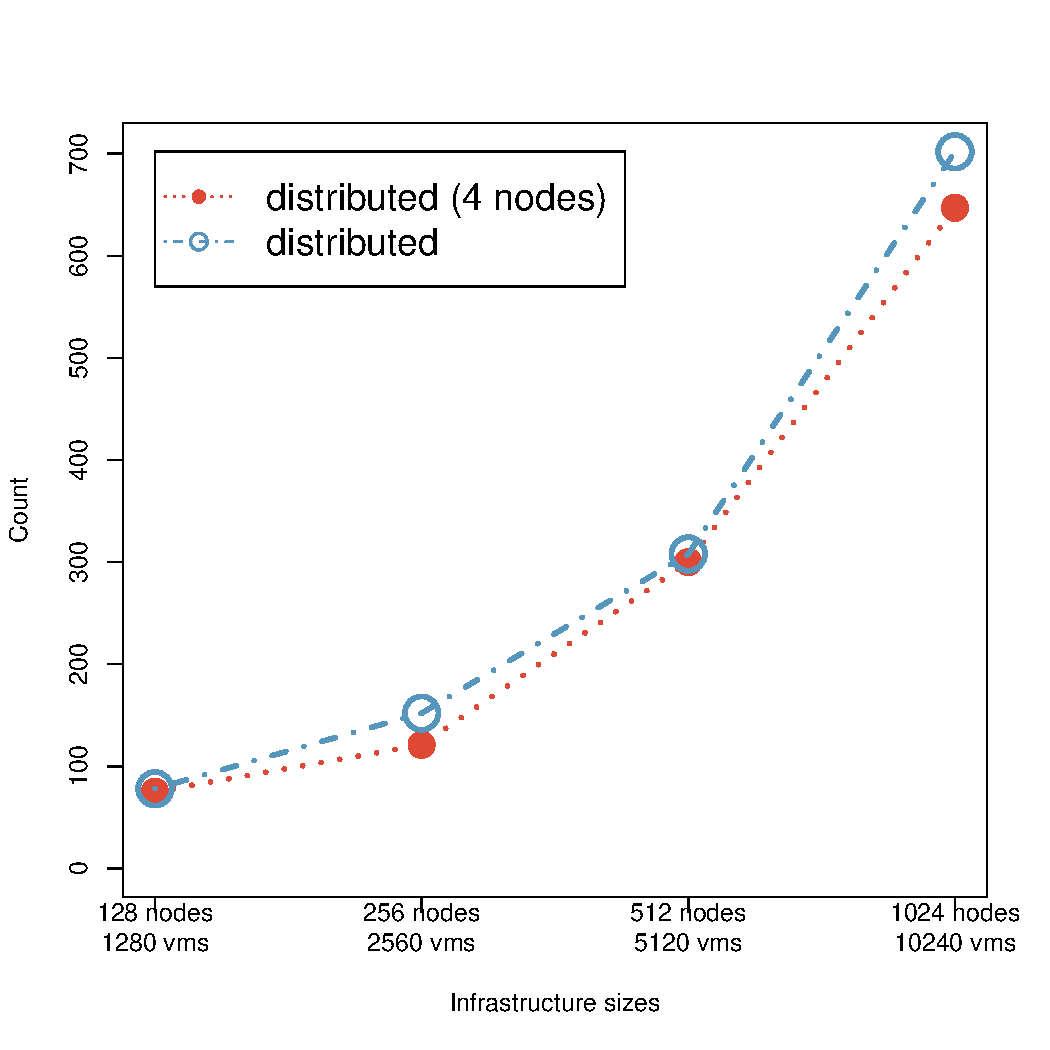
\includegraphics[width=.47\linewidth]{figures/experiments/dvms_comparison_migration_count.pdf}
%   \label{fig:dvms_comparison_migration_count}}
% \subfigure[Cumulated violation duration]{
%   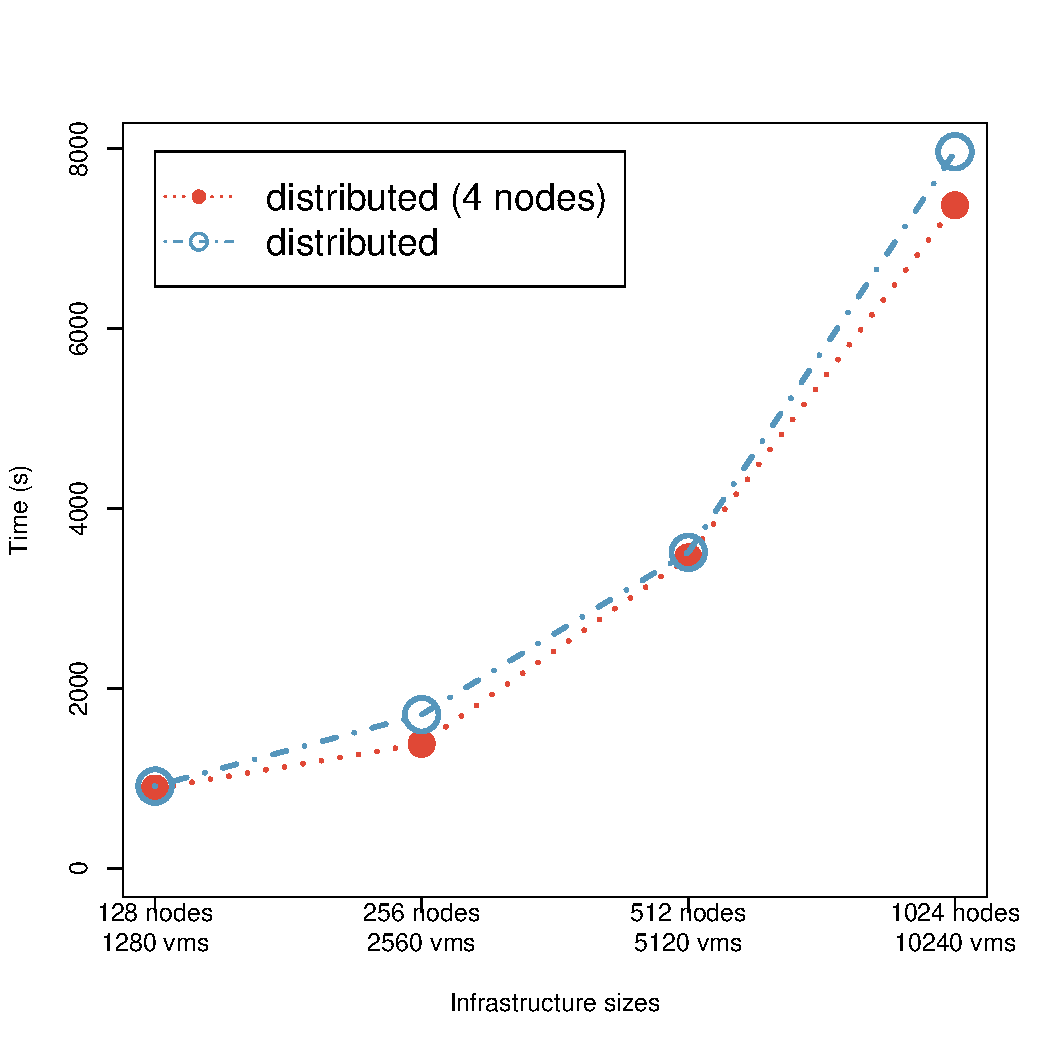
\includegraphics[width=.47\linewidth]{figures/experiments/dvms_comparison_violation_duration.pdf}
%   \label{fig:dvms_comparison_violation_duration}}
% \caption{Comparison of two flavours of DVMS}
% \label{fig:violation_clouds}
% \end{figure}

\begin{table}[ht]
\centering
    {\scriptsize \begin{tabular}{|P{27mm}@{\:}||@{\:}c@{\:}|@{\:}c@{\:}||@{\:}c@{\:}|@{\:}c@{\:}|}
      \thickhline
      \textbf{Infrastructure Size}
        & \multicolumn{2}{c@{\:}||@{\:}}{\textbf{No.\ migrations}}
        & \multicolumn{2}{c@{\:}|}{\textbf{Violation time (s)}}
          \Tstrut \\
         \hfill flavour &  ~Original~ & 4 nodes  &  ~Original~ & 4 nodes \Bstrut \\
      \thickhline

        128 nodes &   78  & 76  & 914.28  & 884.46  \\
        256 nodes &   152 & 127 & 1709.23 & 1498.71 \\
        512 nodes &   308 & 286 & 3513.18 & 3314.72 \\
       1024 nodes &   702 & 616 & 7967.03 & \:7101.49

      \Rstrut  \\ \hline
      \thickhline
  \end{tabular} }
\caption{Comparison of two DVMS flavours.}
\label{tab:dvms_flavours}
\end{table}

% {\scriptsize \begin{tabular}{|P{27mm}@{\:}||@{\:}c@{\:}|@{\:}c@{\:}|@{\:}c@{\:}||@{\:}c@{\:}|@{\:}c@{\:}|@{\:}c@{\:}|}
%     \thickhline
%     \textbf{Algorithm}
%       & \multicolumn{3}{c@{\:}||@{\:}}{\textbf{No.\ migrations}}
%       & \multicolumn{3}{c@{\:}|}{\textbf{Violation time (s)}}
%         \Tstrut \\
%        \hfill\#LCs  & ~128~ & ~256~ & 512 & ~~128~~ & ~~256~~ & 512 \Bstrut \\
%     \thickhline
%       Reactive      & 107 & 201 & 421 & 1075 & 1955 & 4385 \\
%       Periodic 30s  & 62 & 124 & 269 & 1770 & 3453 & \:8196
%     \Rstrut  \\ \hline
%     \thickhline
% \end{tabular}

% \caption{Influence of the Snooze group size ($Med\pm \sigma$)}
% \label{tab:dvms_flavours}
% }


% \begin{figure}[ht]
% \begin{center}
%     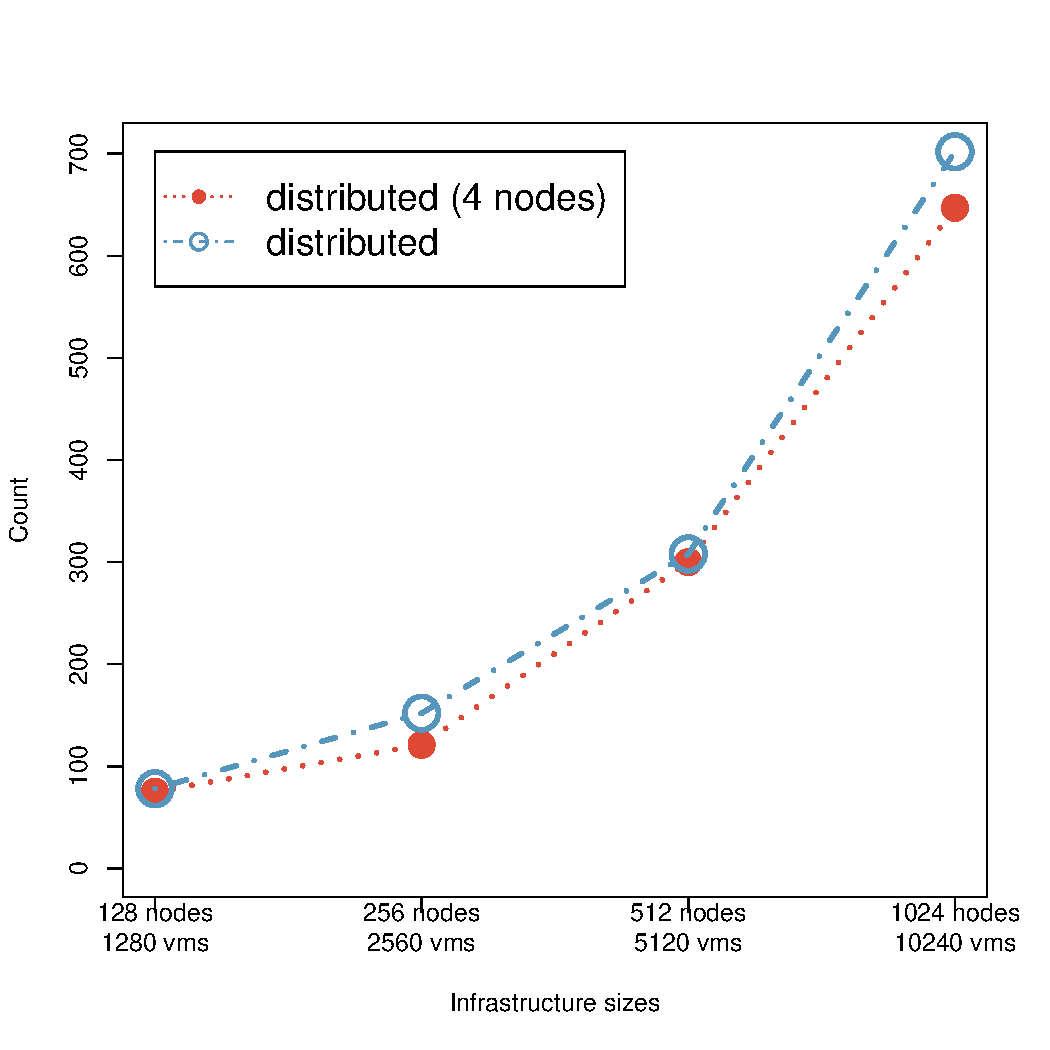
\includegraphics[width=.65\linewidth]{figures/experiments/dvms_comparison_migration_count.pdf}
%     \caption{Comparison of two flavour of DVMS (migration count).}
%     \label{fig:dvms_comparison_migration_count}
% \end{center}
% \end{figure}

In Table \ref{tab:dvms_flavours}, we compared two implementations of
DVMS: one that complies the description given in Section \ref{sec:ISP} and one
that works on partitions which contain at least 4 nodes. It is noticeable that
the number of migrations is slightly smaller with the implementation that works
with at least 4 nodes. This is due to the quality of reconfiguration plans: as
more nodes can be used to rebalance the VMs workload, its quality can be
improved.

% \begin{figure}[ht]
% \begin{center}
%     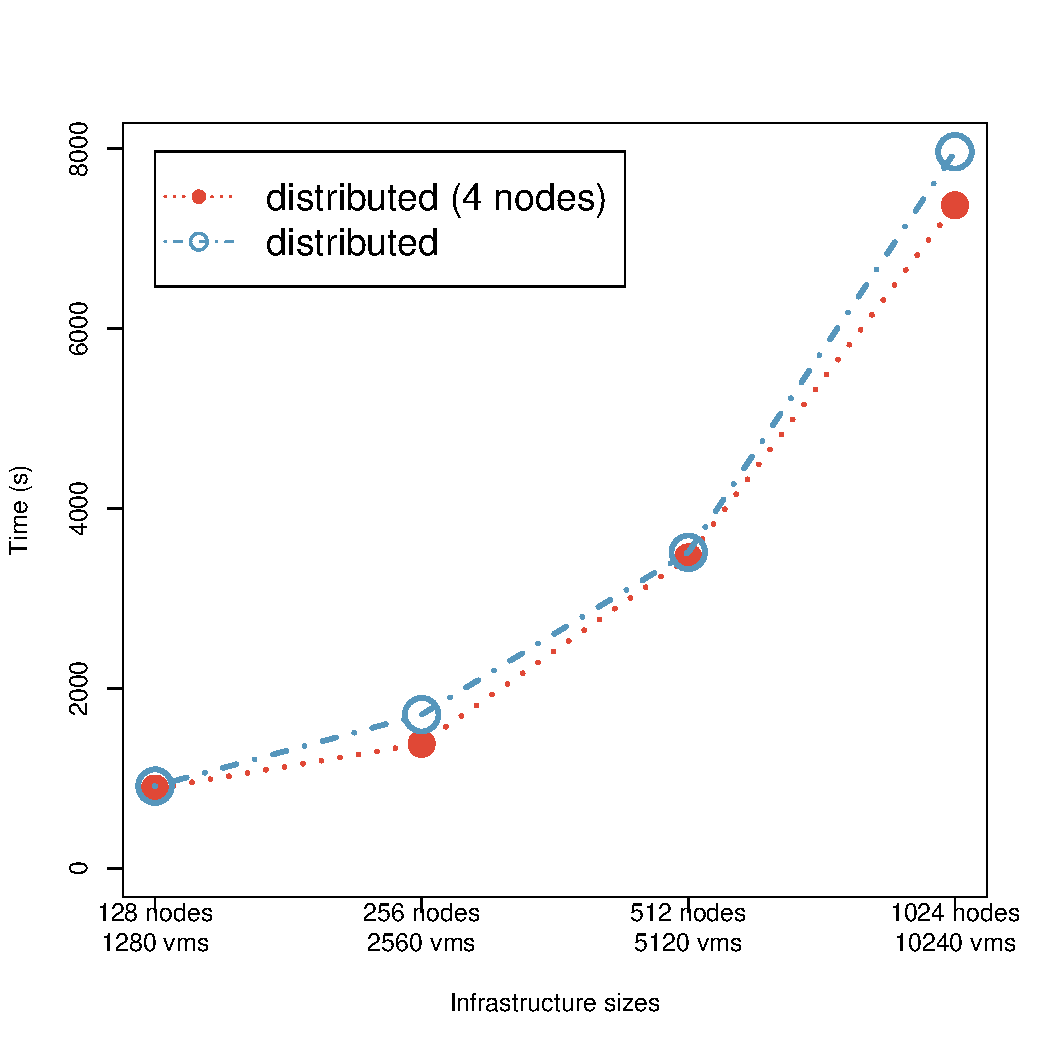
\includegraphics[width=.65\linewidth]{figures/experiments/dvms_comparison_violation_duration.pdf}
%     \caption{Comparison of two flavour of DVMS (cumulated violation time).}
%     \label{fig:dvms_comparison_violation_duration}
% \end{center}
% \end{figure}

Table \ref{tab:dvms_flavours} also shows that the preceding
fact has a direct impact on the VMs QoS: the cumulated violation duration
is reduced in the same proportion as the reduction of migrations.
% The comparison of different flavours of the DVMS algorithm is eased by the use
% of the VMPlaceS framework.


